\documentclass[12pt,fleqn]{article}\usepackage{../../common}
\begin{document}
Sıvılar - 2

Taşınımsal Yer Değişim (Convective Transport)

Bu kavramı anlamak için bir akışın önünde duran geçirgen bir yüzey
düşünelim. Akışı temsil eden hız alanını biliyoruz, bu alanın yüzeydeki
vektörleri bir sıvı parçacığının o noktadaki, o andaki hareketini gösteriyor.

Bir sıvı parçacığı yeri değiştirilebilecek belli oranda bir madde, öğe
içerebilir, ve o parçacık yüzeyin bir tarafından diğer tarafına geçtiğinde
parçacıkli beraber ögenin yeri de değişmiş olur. Dikkat yer değişimi direk bir
geçiş ima eder, hızın normal bileşenine oranla bir geçiştir bu. Bu bağlamda
hızın sadece normal (yüzeye dik) olan bileşenine bakarız, çünkü yüzeye
teğet olan bileşen hiç bir geçiş oluşturmazdı, yüzeye paralel olan bir
gidiştir bu. Tabii ki yüzeyin farklı noktalarında farklı hızlar, ve farklı
öğe değerleri olabilir, bu sebeple taşınmsal yer değişiminin matematiksel
tarifi bu farklılıkları göz önüne almalıdır. 

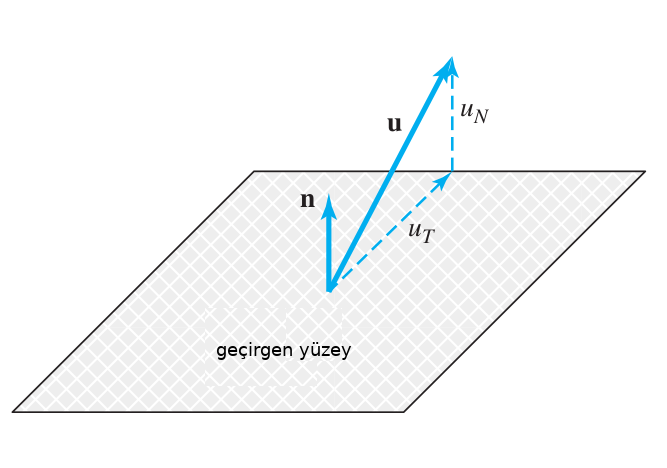
\includegraphics[width=20em]{phy_030_fluid2_04.png}










[devam edecek]


Doğu-Batı yönü E,W ile Kuzey-Güney yönü N,S ile Yukarı-Aşağı yönü T,S
ile belirtilecek. 

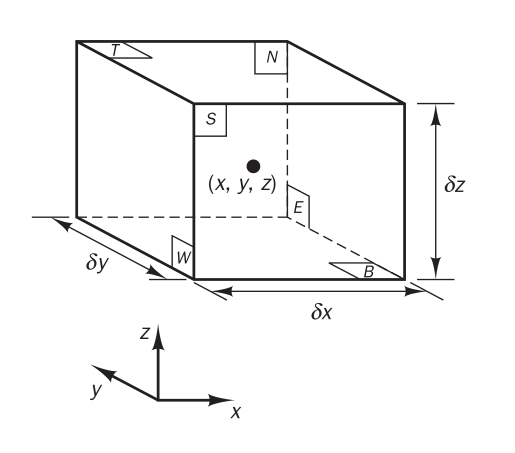
\includegraphics[width=15em]{phy_030_fluid2_03.png}

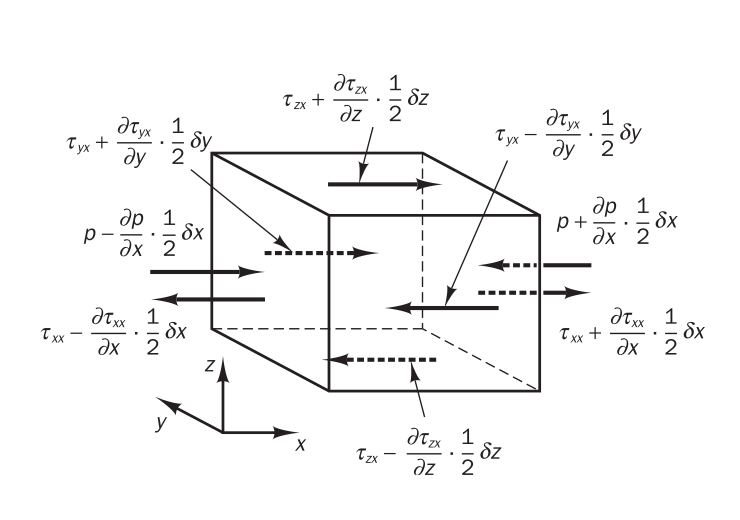
\includegraphics[width=20em]{phy_030_fluid2_01.png}

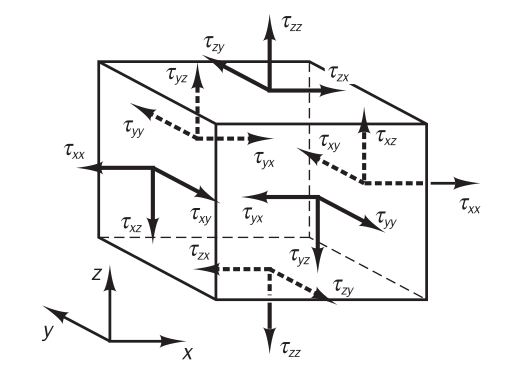
\includegraphics[width=15em]{phy_030_fluid2_02.png}


Ornek olarak $x$ yonundeki kuvvetleri her uc yon icin hesaplayalim.

$E,W$ yüzleri üzerindeki $x$ kuvvetleri, 

$$
\left[
  \left( p - \frac{\partial p}{\partial x} \frac{1}{2} \delta x \right) -
  \left( \tau_{xx} - \frac{\partial \tau_{xx}}{\partial x} \frac{1}{2} \delta x \right) 
\right]
  \delta y \delta z  +
\left[
  -\left( p + \frac{\partial p}{\partial x} \frac{1}{2} \delta x \right) +
  \left( \tau_{xx} + \frac{\partial \tau_{xx}}{\partial x} \frac{1}{2} \delta x \right) 
  \delta y \delta z  +  
\right]
$$

$$
= \left(
-\frac{\partial p}{\partial x} + \frac{\partial \tau_{xx}}{\partial x}
\right)
\delta x \delta y \delta z
$$

$N,S$ yönündekiler,

$$
- \left( \tau_{yx} - \frac{\partial \tau_{yx}}{\partial y}  \frac{1}{2} \delta y
\right) \delta x \delta z  +
\left( \tau_{yx} - \frac{\partial \tau_{yx}}{\partial y}  \frac{1}{2} \delta y
\right) \delta x \delta z  
$$

$$
= \frac{\partial \tau_{yx}}{\partial y} \delta x \delta y \delta z 
$$

$T,B$ üzerindekiler,

$$
- \left(
\tau_{zx} - \frac{\partial \tau_{zx}}{\partial z} \frac{1}{2} \delta z
\right) \delta x \delta y +
\left(
\tau_{zx} + \frac{\partial \tau_{zx}}{\partial z} \frac{1}{2} \delta z
\right) \delta x \delta y 
$$

$$
= \frac{\partial \tau_{zx}}{\partial z} \delta x \delta y \delta z 
$$

Birim hacimdeki üstteki yüzey streslerinin etkisi için üstteki üç sonucu
toplayıp $\delta x \delta y \delta z $ ile böleriz, sonuç,

$$
\frac{\partial (-p + \tau_{xx})}{\delta x} +
\frac{\partial \tau_{yx}}{\partial y} +
\frac{\partial \tau_{zx}}{\partial z} 
$$






[devam edecek]

Kaynaklar

[1] Versteeg, {\em An Introduction to CFD}

[2] Katz, {\em Introduction to Fluid Mechanics}

\end{document}
